% Quantum Machine Intelligence (Springer) submission.
% Format: standard article + natbib author-year (Springer template optional;
% production re-typesets). Single-blind: author names included.
\documentclass[11pt]{article}

\usepackage[margin=1.1in]{geometry}
\usepackage{amsmath,amssymb,amsfonts}
\usepackage{graphicx}
\usepackage{booktabs}
\usepackage{multirow}
\usepackage[round]{natbib}
\usepackage{xurl}
\usepackage[hidelinks]{hyperref}
\usepackage{microtype}
\usepackage{authblk}

\newcommand{\ket}[1]{\left|#1\right\rangle}
\newcommand{\bra}[1]{\left\langle#1\right|}
\newcommand{\expect}[1]{\langle#1\rangle}
\newcommand{\Hnoisy}{\expect{H}_{\mathrm{noisy}}}
\newcommand{\Hideal}{\expect{H}_{\mathrm{ideal}}}
% table* is a two-column float in IEEE; map it to table here so the
% generated tables compile unchanged in one-column layout.
\makeatletter
\let\table@star\table
\expandafter\def\csname table*\endcsname{\table}
\expandafter\def\csname endtable*\endcsname{\endtable}
\makeatother

\title{Budget-Aware Neural Error Mitigation for\\ Variational Quantum Algorithms}

\author[1]{Guilin Zhang}
\author[1]{Kai Zhao}
\author[1]{Xu Chu}
\affil[1]{Workday AI Research}

\date{}

\begin{document}
\maketitle

\begin{abstract}
Quantum error mitigation methods differ not only in accuracy but in how many quantum circuit executions they consume per estimate: zero-noise extrapolation (ZNE) requires 3--5 executions, Clifford data regression (CDR) requires more than 30 per target circuit, while a trained neural mitigator needs exactly one. We argue that the practically relevant comparison is at \emph{equal total shot budget per evaluation point}, the regime faced by every variational quantum algorithm (VQA) whose optimization loop must evaluate thousands of parameter settings. We present a budget-conditioned neural error mitigation (NEM) model that predicts ideal expectation values from a single shot-limited measurement, circuit features, and device-characterization features, with the shot-noise scale supplied as an input so one network serves all budgets. Under an equal-budget protocol in which every method---including each ZNE fold point and each CDR training circuit---consumes measured shots under the same frozen noise realization, NEM is the only method that improves on unmitigated execution at budgets up to $2^{14}$ shots in both noise regimes studied, reducing error by 72--81\% under combined stochastic and coherent-miscalibration noise; CDR overtakes NEM only at $2^{16}$ shots per evaluation. We further characterize when extrapolation fails: under physically motivated control-offset miscalibration, folding-based ZNE returns a worse answer than no mitigation on roughly half of all instances, with unbounded single-instance errors, while NEM degrades gracefully and CDR remains accurate at $32\times$ the quantum cost. We confirm this failure on a real IBM Heron processor, where folding ZNE returns a worse answer than no mitigation on up to 88\% of instances. Under structured noise, the neural improvements persist without degradation from 4 to 20 qubits. Budget-aware accounting, we argue, is the comparison that matters for deployment.

\medskip
\noindent\textbf{Keywords:} quantum error mitigation, variational quantum algorithms, neural networks, NISQ, zero-noise extrapolation, Clifford data regression
\end{abstract}

\section{Introduction}
\label{sec:intro}

Variational quantum algorithms such as the variational quantum eigensolver (VQE) and the quantum approximate optimization algorithm (QAOA) are leading candidates for near-term quantum advantage, but their expectation-value estimates are biased by device noise \citep{preskill2018quantum,cerezo2021variational,bharti2022noisy,tilly2022variational}. Error mitigation aims to remove this bias without the qubit overhead of error correction \citep{temme2017error,cai2023quantum}. The most widely used technique, zero-noise extrapolation, amplifies noise by gate folding and extrapolates measurements to the zero-noise limit \citep{temme2017error,li2017efficient,giurgicatiron2020digital,kim2023evidence}; learning-based methods such as Clifford data regression instead fit a noisy-to-ideal map on classically simulable circuits executed on the same device \citep{czarnik2021error,strikis2021learning}.

These methods are usually compared at a fixed, often generous, number of measurement shots \emph{per circuit execution}. This obscures a first-order practical distinction: ZNE consumes 3--5 circuit executions per mitigated estimate, and CDR consumes one execution per training circuit (typically more than 30) \emph{for every new target circuit}, while a neural model trained offline consumes exactly one. Inside a VQA optimization loop that evaluates thousands of parameter settings under a per-iteration shot budget, these multiplicities---not the asymptotic accuracy at unlimited shots---decide which method is usable. \citet{bultrini2023unifying} made the budget axis explicit for classical mitigation methods and found that the method ranking is budget-dependent; we extend that analysis to learned mitigation and make the budget an input of the model itself.

This paper makes four contributions.

\emph{(i) Budget-conditioned neural mitigation.} We train a neural error mitigation model that maps a single $S$-shot measured estimate, circuit-structure features, and device-characterization features to the ideal expectation value, and we condition it on the shot-noise scale $1/\sqrt{S}$ so that one network serves every budget (Section~\ref{sec:method}).

\emph{(ii) An equal-budget evaluation protocol and Pareto analysis.} Every method receives the same total shot budget $B$ per evaluation point, split across the executions it requires, with every execution---including each ZNE fold point and each CDR training circuit---drawn as measured shots under the same frozen noise realization (Section~\ref{sec:setup}). Under this protocol NEM is the only method that beats unmitigated execution at $B\le 2^{14}$ in both regimes studied, and CDR overtakes it only at $B=2^{16}$ (Section~\ref{sec:pareto}).

\emph{(iii) A characterization of extrapolation failure.} Under physically motivated control-offset miscalibration \citep{krantz2019engineer}, unitary folding amplifies the coherent angle error linearly while the observable responds non-monotonically, so ZNE underperforms unmitigated execution on 38--65\% of instances with unbounded single-instance error; we map the failure boundary as a function of the miscalibration strength and quantify tail risk (Section~\ref{sec:failure}), and we confirm the failure on a real IBM Heron processor (Section~\ref{sec:hardware}).

\emph{(iv) Scaling and controls.} Mean error reductions of 61--85\% under structured noise persist without degradation from 4 to 20 qubits, and a direct-prediction control---predicting $\Hideal$ from features alone, without the noisy measurement---fails catastrophically at every size, confirming that mitigation, not memorization, drives the result (Sections~\ref{sec:scaling} and~\ref{sec:ablations}).

We are explicit about what NEM does not win: given $32\times$ the per-evaluation quantum budget, CDR is the most accurate method in every regime we study. The case for learned mitigation is not accuracy supremacy but its position on the budget--accuracy Pareto frontier and its bounded failure behavior.

\section{Related work}
\label{sec:related}

\paragraph{Classical mitigation.}
ZNE \citep{temme2017error,li2017efficient} assumes the bias varies smoothly with a controllable noise-scale factor; digital implementations amplify noise by unitary folding \citep{giurgicatiron2020digital}, and the technique has produced headline demonstrations on hardware at the 100-qubit scale \citep{kim2023evidence}. Its reliability, however, is contingent on the extrapolation ansatz matching the actual noise response, a sensitivity we quantify in Section~\ref{sec:failure}. Probabilistic error cancellation \citep{temme2017error,van2023probabilistic} yields unbiased estimates at exponential sampling cost; virtual distillation \citep{huggins2021virtual,koczor2021exponential} suppresses errors using multiple state copies at additional quantum cost. CDR \citep{czarnik2021error} fits a linear noisy-to-ideal regression on near-Clifford circuits executed on the device, paying tens of executions per target circuit but inheriting robustness to noise structure because it calibrates on the device as it actually is; \citet{strikis2021learning} extend the idea with learning-based protocols. \citet{bultrini2023unifying} benchmark these methods under a unified framework as a function of total shot budget and find that cheap methods win at small budgets while data-hungry methods win at large ones---the organizing observation our protocol builds on.

\paragraph{Learned mitigation.}
Neural networks have been used to reconstruct states and observables from noisy quantum data \citep{torlai2018neural} and to mitigate errors in quantum simulation \citep{bennewitz2022neural}. \citet{liao2023machine} benchmark random forests, multilayer perceptrons, and graph networks for expectation-value mitigation, including at the 100-qubit scale on hardware, and find learned models competitive with ZNE at lower quantum cost---an observation our protocol makes systematic. Closest to this work, \citet{cantori2024synergy} train convolutional networks to predict ideal expectation values of parameterized circuits from noisy values and circuit structure, including transfer to circuit sizes beyond the training set, and \citet{liao2025noiseagnostic} train noise-agnostic models with data-augmented training, outperforming ZNE and CDR on hardware at 4--6 qubits. In this journal, \citet{adeniyi2025adaptive} adapt a neural mitigator to per-circuit error characteristics and validate it on IBM hardware. Neither line of work controls for quantum cost: comparisons grant every method full per-execution shot counts, and the per-evaluation execution multiplicity is not part of the analysis. Our contribution is orthogonal and composable with theirs: an equal-budget protocol, budget conditioning of the model itself, and an explicit failure-mode analysis of the classical alternative.

\section{Budget-conditioned neural mitigation}
\label{sec:method}

A VQA prepares $\ket{\psi(\boldsymbol{\theta})}=U(\boldsymbol{\theta})\ket{0}^{\otimes n}$ and estimates the objective $C(\boldsymbol{\theta})=\bra{\psi(\boldsymbol{\theta})}H\ket{\psi(\boldsymbol{\theta})}$. On hardware one observes an $S$-shot estimate of the noisy expectation,
\begin{equation}
\widehat{\expect{H}}_{\mathrm{noisy}} \;=\; \Hideal + \delta(\boldsymbol{\theta},\mathcal{E}) + \varepsilon_S,
\end{equation}
where $\delta$ is the bias induced by the noise process $\mathcal{E}$ and $\varepsilon_S$ is measurement noise with scale proportional to $1/\sqrt{S}$. We learn a correction function
\begin{equation}
f_\phi\!\left(\widehat{\expect{H}}_{\mathrm{noisy}},\, \mathbf{x}_c,\, \mathbf{x}_n,\, 1/\sqrt{S}\right) \;\approx\; \Hideal ,
\label{eq:model}
\end{equation}
where $\mathbf{x}_c$ collects circuit features (qubit count, layer count, parameter count, and the variational angles themselves; dimension $3+4n$ for the ansatz family used here) and $\mathbf{x}_n$ collects device-characterization features (gate error rates, readout asymmetries, and---when characterized---the calibration-drift scale; Section~\ref{sec:setup}).

\begin{figure}[t]
\centering
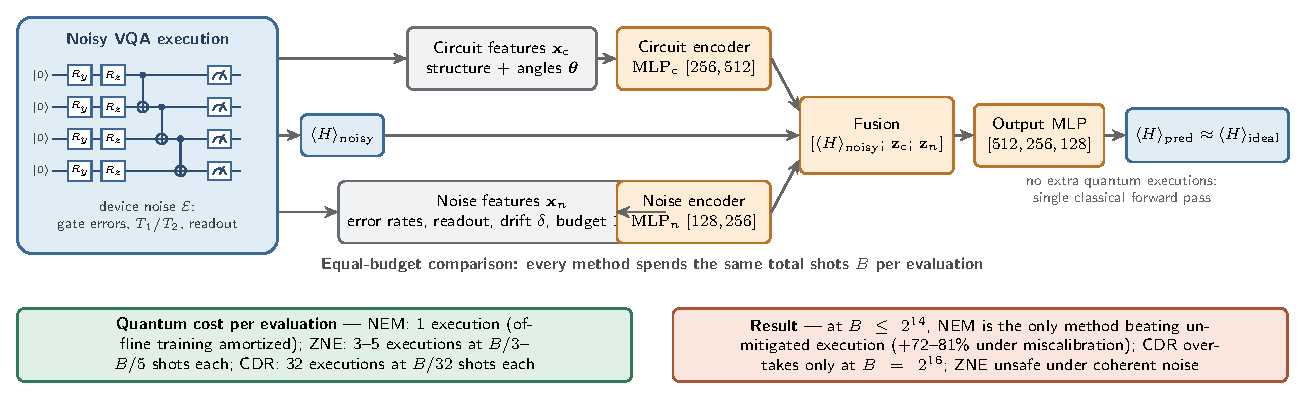
\includegraphics[width=\textwidth]{figures/overview_diagram.pdf}
\caption{Budget-conditioned neural error mitigation. A single $S$-shot noisy VQA execution is combined with circuit-structure and device-characterization embeddings---including the shot-noise scale $1/\sqrt{S}$---to predict the ideal expectation value with one classical forward pass. Under an equal total budget $B$ per evaluation point, competing methods must split $B$ across their 3--32 required executions.}
\label{fig:overview}
\end{figure}

\paragraph{Architecture.}
Figure~\ref{fig:overview} shows the model. Two multilayer-perceptron encoders embed the feature groups: the circuit encoder maps $\mathbf{x}_c$ through hidden widths $[128,256]$ to a 128-dimensional embedding, and the noise encoder maps $\mathbf{x}_n$ through width 64 to a 64-dimensional embedding. The embeddings are concatenated with the measured value and passed through an output network of widths $[256,512,256]$ (LayerNorm, GELU, dropout $0.15$) that predicts a residual correction added to the input estimate. The standard configuration has 428K parameters; Section~\ref{sec:ablations} shows accuracy is insensitive to capacity over a $5\times$ range, so the capacity is generous rather than necessary.

\paragraph{Training.}
The model minimizes the Huber loss with AdamW (learning rate $10^{-3}$, weight decay $10^{-4}$, cosine annealing with warm restarts) for 75 epochs---about five minutes on a CPU workstation at the sizes studied. Training pairs $(\widehat{\expect{H}}_{\mathrm{noisy}}, \mathbf{x}_c, \mathbf{x}_n, \Hideal)$ are generated in simulation: parameters and noise realizations are sampled per example, the noisy input is an actual $S$-shot measured estimate, and the ideal label is computed by exact noiseless simulation. Ideal labels therefore restrict \emph{training} to classically simulable sizes, a limitation we return to in Section~\ref{sec:discussion}.

\paragraph{Budget conditioning.}
Each training example draws its shot count $S$ log-uniformly from $2^{8}$ to $2^{16}$, samples the noisy input at that $S$, and appends $1/\sqrt{S}$ to $\mathbf{x}_n$. The network thereby learns how much of the input fluctuation is measurement noise versus learnable bias---at small $S$ it shrinks its trust in the measurement, at large $S$ it corrects fine structure---and a single model serves every deployment budget without retraining.

\paragraph{Costs.}
Data generation is a one-time cost of 4{,}400 circuit executions per device and noise regime, amortized over every subsequent evaluation; inference adds one classical forward pass (under one millisecond) to a single quantum execution. Table~\ref{tab:cost} summarizes per-evaluation costs against the baselines.

\begin{table}[t]
\caption{Per-evaluation quantum cost at total budget $B$.}
\label{tab:cost}
\centering
\small
\begin{tabular}{lccc}
\toprule
Method & Executions & Shots per execution & Offline cost \\
\midrule
Unmitigated & 1 & $B$ & --- \\
NEM (ours) & 1 & $B$ & 4.4K executions $+$ 5 min training \\
ZNE (exponential) & 3 & $B/3$ & --- \\
ZNE (adaptive) & 4 & $B/4$ & --- \\
CDR & 32 & $B/32$ & repeated per target circuit \\
\bottomrule
\end{tabular}
\end{table}

\paragraph{Break-even.}
The offline cost is recovered after a modest number of evaluations. Let $M$ be the number of distinct evaluation points---parameter settings, or target circuits---that a deployed model serves before retraining. Counting every execution at equal per-execution shots, NEM's total quantum cost is $4400 + M$, against $kM$ for ZNE ($k=3$ or $4$) and $32M$ for CDR; the baselines carry no offline cost but pay their multiplicity at \emph{every} point, since CDR re-fits its near-Clifford regression for each target circuit. NEM is cheaper in total once $M$ exceeds $M^\star = \lceil 4400/(k-1) \rceil$: 142 points relative to CDR, 1{,}467 relative to adaptive ZNE, and 2{,}200 relative to exponential ZNE (Table~\ref{tab:breakeven}). A VQE optimization loop evaluates $10^3$--$10^4$ parameter settings, so it clears the CDR break-even by one to two orders of magnitude within a single run. The bound is conservative: training shots are drawn from $2^8$--$2^{16}$, so a deployment budget $B>2^8$ per execution amortizes the offline cost faster still.

\begin{table}[t]
\caption{Break-even: distinct evaluation points $M^\star$ beyond which NEM's total quantum cost (offline plus one execution per point) falls below the baseline's.}
\label{tab:breakeven}
\centering
\small
\begin{tabular}{lcc}
\toprule
NEM vs.\ & Per-eval.\ executions & Break-even $M^\star$ \\
\midrule
ZNE (exponential) & 3 & 2{,}200 \\
ZNE (adaptive) & 4 & 1{,}467 \\
CDR & 32 & 142 \\
\bottomrule
\end{tabular}
\end{table}

\section{Experimental protocol}
\label{sec:setup}

\paragraph{Circuits and observables.}
We use hardware-efficient VQE ansatzes (alternating $R_Y,R_Z$ rotation layers and CNOT ladders, two layers) at $n=4$--$16$ qubits with the mean-magnetization observable $H=\frac{1}{n}\sum_i Z_i$. Simulations use Qiskit Aer \citep{qiskit2024}: exact density-matrix count sampling up to 10 qubits and statevector trajectory sampling above, so every reported measurement carries genuine sampling statistics. Classical baselines use mitiq~1.0 \citep{larose2022mitiq}.

\paragraph{Noise regimes.}
Three regimes span the noise-structure spectrum:
\begin{itemize}
\item \emph{Stochastic device noise}: per-instance device profiles (depolarizing gate errors, thermal relaxation, asymmetric readout) sampled over realistic ranges---the regime where smooth noise-scaling assumptions are most plausible.
\item \emph{Stochastic-correlated noise}: adds per-instance gate-error fluctuations and correlated $ZZ$ crosstalk.
\item \emph{Coherent miscalibration}: models control-offset calibration error \citep{krantz2019engineer}. Working in the native gate basis $\{R_Z,\sqrt{X},X,\mathrm{CNOT}\}$, every physical pulse executes its nominal angle plus an offset drawn once per device snapshot from $\mathcal{N}(\delta,(\delta/2)^2)$ with $\delta\in[0.02,0.06]$\,rad, on top of two-qubit depolarizing noise and asymmetric readout. Virtual $R_Z$ rotations, implemented as exact software frame updates, are exempt. Because the miscalibration lives in the executed unitary, folded ZNE circuits and CDR training circuits face \emph{the same} quantum process. Under folding, offsets in the inverted segment do not cancel---$R_Y(\theta{+}\delta)\,R_Y(-\theta{+}\delta)=R_Y(2\delta)$---so the coherent error grows linearly with the scale factor while the observable responds non-monotonically: the mechanism by which coherent errors defeat extrapolation.
\end{itemize}

\paragraph{Fairness protocol.}
Each test instance freezes one noise realization (a device snapshot). The raw measurement, the NEM input, every ZNE fold point, and every CDR training circuit are $S$-shot measured estimates under that same realization; ideal values are exact noiseless simulations. Baseline failures abort the run; there are no silent fallbacks. ZNE uses mitiq's Richardson, exponential ($y(\lambda)=a\,e^{-b\lambda}$ with the depolarizing asymptote), and adaptive-exponential factories with global folding at scale factors $\{1,2,3\}$; CDR uses 31 near-Clifford training circuits with half the non-Clifford gates retained. We report 150 test instances per configuration (100 for budget sweeps) and paired $t$-tests against unmitigated execution, and because extrapolation has heavy-tailed failures we report median absolute errors alongside means throughout.

\section{Results}
\label{sec:results}

\subsection{The equal-budget Pareto frontier}
\label{sec:pareto}

\begin{figure}[t]
\centering
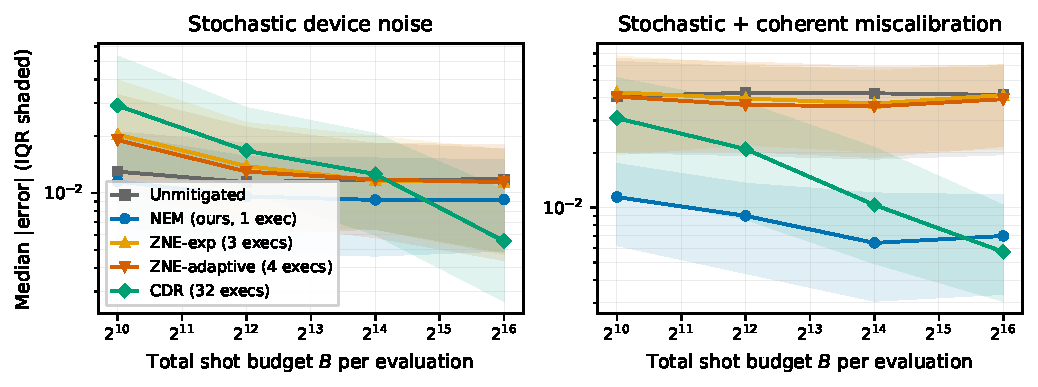
\includegraphics[width=\textwidth]{figures/budget_pareto.pdf}
\caption{Equal-budget comparison at $n=8$ (100 instances; median $|$error$|$, interquartile range shaded). Every method spends the same total budget $B$ per evaluation point, split across its required executions (Table~\ref{tab:cost}). NEM is the only method below the unmitigated baseline at $B\le2^{14}$ in both regimes; CDR crosses over only at the largest budget. ZNE medians track the unmitigated line: for the typical instance extrapolation removes nothing, while its mean error diverges (Section~\ref{sec:failure}).}
\label{fig:pareto}
\end{figure}

Figure~\ref{fig:pareto} shows the central result; Table~\ref{tab:budget_full} in the appendix lists every value. Under coherent-miscalibration noise, NEM reduces the mean error by 72\%, 77\%, 81\%, and 81\% at $B=2^{10},2^{12},2^{14},2^{16}$ respectively---flat in $B$, because the learned correction targets the systematic bias and its training cost is already amortized. CDR, whose per-execution shot count is $B/32$, climbs from $+23\%$ at $B=2^{10}$ to $+84\%$ at $B=2^{16}$, overtaking NEM only at the largest budget. Both ZNE variants are \emph{negative} at every budget in this regime ($-36\%$ to $-471\%$ in the mean). Under stochastic device noise the picture compresses (the residual error is dominated by shot noise), but the ordering at low budget is the same: NEM is the only positive method at $B\le2^{14}$ ($+11$ to $+20\%$), and CDR turns positive only at $B=2^{16}$ ($+47\%$).

The practical reading is direct. A VQE optimization loop evaluating $10^3$--$10^4$ parameter settings at a realistic per-iteration budget of $10^3$--$10^4$ shots sits squarely in the regime where single-execution learned mitigation is the only option that helps at all; per-instance methods become competitive only when the per-evaluation budget grows by more than an order of magnitude.

\subsection{When extrapolation fails, and how badly}
\label{sec:failure}

\begin{figure}[t]
\centering
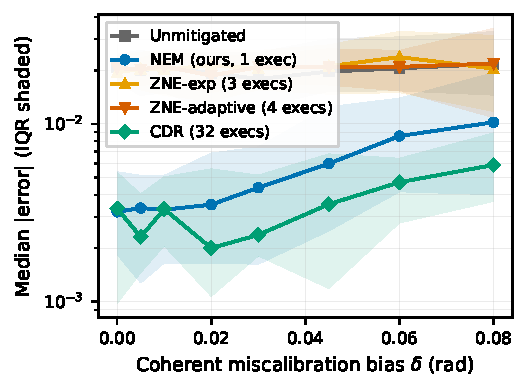
\includegraphics[width=0.62\textwidth]{figures/phase_boundary.pdf}
\caption{Median $|$error$|$ versus miscalibration strength $\delta$ at $n=8$ (80 instances per point, 8{,}192 shots per execution). ZNE medians coincide with the unmitigated baseline at every $\delta$, including $\delta=0$, where the residual bias is dominated by readout error that folding does not amplify. NEM matches CDR at small $\delta$ at $1/32$ the quantum cost, and its improvement declines smoothly as the unlearnable coherent share grows.}
\label{fig:boundary}
\end{figure}

Figure~\ref{fig:boundary} sweeps the coherent bias $\delta$ from 0 to 0.08\,rad over a fixed stochastic background. Three observations follow.

First, ZNE's \emph{median} improvement never exceeds $+2\%$ anywhere on the sweep---including at $\delta=0$, because the remaining bias there is dominated by readout error, which gate folding does not amplify; extrapolation removes the gate-error component and faithfully retains the rest.

Second, ZNE's \emph{mean} error explodes as $\delta$ grows (for exponential extrapolation, $-646\%$ at $\delta=0.06$), driven by heavy tails. Table~\ref{tab:safety} shows the anatomy at one representative cell, and Table~\ref{tab:safety_full} in the appendix shows every structured-regime cell: ZNE returns a result worse than the unmitigated estimate on 38--65\% of instances, with single-instance errors reaching three orders of magnitude above the unmitigated level when the extrapolation fit diverges. Extrapolation is an unbounded operation: at $n{=}12$ we observe a single instance where the adaptive variant's error reaches $371$ in observable units, more than three orders of magnitude above the worst unmitigated error in that cell.

Third, NEM tracks CDR at small $\delta$ ($+82\%$ versus $+83\%$ mean at $\delta=0$) at $1/32$ of the quantum cost; its improvement declines smoothly to $+44\%$ at $\delta=0.08$ as the high-dimensional oscillatory component of the coherent bias exceeds what the network can learn from 4{,}000 samples. CDR, which re-fits per instance, stays at 69--86\%.

\begin{table}[t]
\caption{Robustness statistics, coherent-miscalibration regime, $n{=}10$ (150 instances, 8{,}192 shots per execution). ``Worse'' is the fraction of instances on which the method's error exceeds the unmitigated error.}
\label{tab:safety}
\centering
\small
\begin{tabular}{lccccc}
\toprule
Method & Mean & Median & p95 & Max & Worse \\
\midrule
Unmitigated & .0412 & .0385 & .080 & 0.11 & --- \\
NEM (ours) & \textbf{.0061} & \textbf{.0044} & \textbf{.015} & \textbf{0.03} & 7\% \\
ZNE-Richardson & .0460 & .0432 & .099 & 0.15 & 63\% \\
ZNE-exponential & .1569 & .0385 & .081 & 17.1 & 49\% \\
ZNE-adaptive & .1220 & .0394 & .082 & 12.1 & 53\% \\
CDR ($32\times$ cost) & .0035 & .0025 & .009 & 0.01 & 6\% \\
\bottomrule
\end{tabular}
\end{table}

The asymmetry in failure behavior matters as much as the averages. The neural model's output is a bounded residual correction: across all 2{,}000 structured-regime test instances (4--20 qubits) its worst-case error stays \emph{below} the worst unmitigated error, in every cell. A simple ensemble safeguard---train three seeds, fall back to the raw value when they disagree beyond a threshold calibrated on unlabeled data---further reduces the worse-than-raw rate from 7\% to 5\% at a cost of three points of mean improvement, and in the low-noise stochastic regime it pins the model's worst case exactly at the unmitigated level. We view the safeguard as cheap insurance rather than a core mechanism.

\subsection{Real-hardware validation}
\label{sec:hardware}

The failure analysis above is the paper's most consequential claim, so we test it on a real device. We run the hardware-efficient VQE on \texttt{ibm\_marrakesh}, a 156-qubit Heron~r2 superconducting processor, on four qubits at two circuit depths (2 and 5 ansatz layers), comparing unmitigated execution against folding ZNE under the equal-budget protocol; ten and eight test instances respectively, 8{,}192 shots, all jobs grouped in a single batch. Real devices carry intrinsic control-offset miscalibration, so no noise is injected---the device \emph{is} the noise source.

Figure~\ref{fig:hardware} shows the result: folding ZNE fails on real silicon exactly as predicted. Its mean error is $3.0\times$ the unmitigated error at two layers and $4.1\times$ at five layers, and it returns a worse answer than no mitigation on 80\% and 88\% of instances respectively. Unitary folding triples the circuit and amplifies the device's coherent and readout errors, which do not extrapolate to the zero-noise limit; the deeper circuit, with more gates to fold, fails harder. This is the same mechanism our simulations isolate (Section~\ref{sec:failure}), now confirmed on hardware without any modelling assumptions. The result establishes that the unsafe regime we characterize is not a simulation artefact but a property of real devices.

This run validates the failure analysis; it is not a hardware-accuracy claim for the neural mitigator, whose improvements we establish in simulation. On these near-shot-noise-floor four-qubit circuits a twin-trained model exhibits a sim-to-real gap, which we analyze in Appendix~\ref{app:hardware} and connect to on-device training~\citep{liao2025noiseagnostic,adeniyi2025adaptive}. Even there the neural correction is \emph{bounded}---it degrades less than ZNE and the safeguard gates it to the unmitigated baseline---whereas folding ZNE amplifies error without bound, the asymmetry this paper emphasizes.

\begin{figure}[t]
\centering
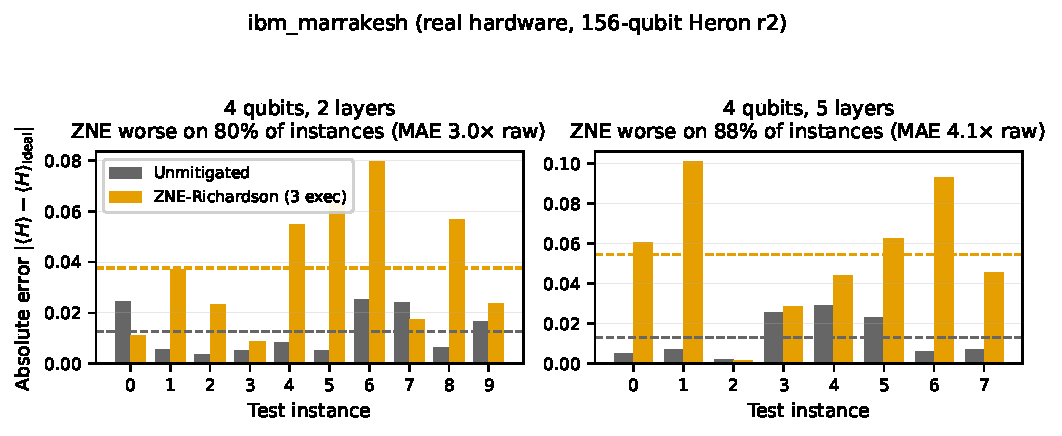
\includegraphics[width=\columnwidth]{figures/hardware_zne.pdf}
\caption{Folding ZNE on real hardware (\texttt{ibm\_marrakesh}, 4 qubits). Per-instance absolute error of unmitigated execution (grey) versus ZNE-Richardson (orange); dashed lines are the means. ZNE's error exceeds the unmitigated error on 80\% (2 layers) and 88\% (5 layers) of instances, with mean error $3.0\times$ and $4.1\times$ the unmitigated level---the failure mode of Section~\ref{sec:failure}, confirmed on a physical device.}
\label{fig:hardware}
\end{figure}

\subsection{Scaling}
\label{sec:scaling}

\begin{figure}[t]
\centering
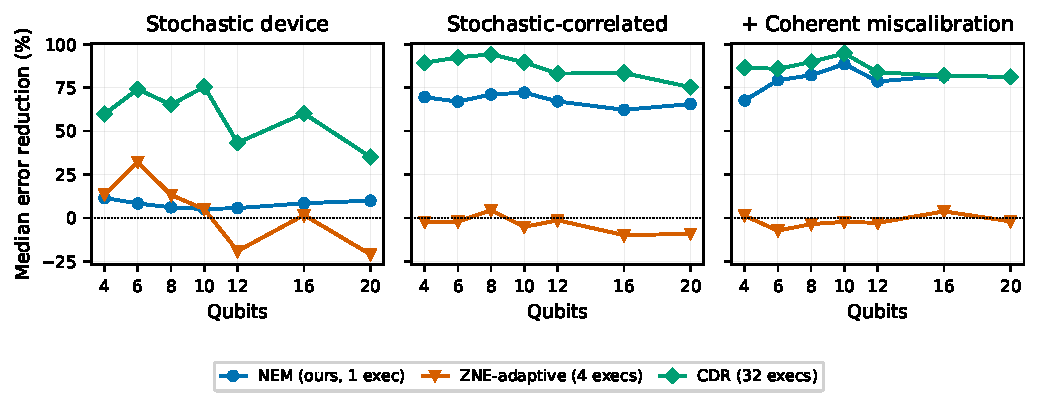
\includegraphics[width=\textwidth]{figures/scaling.pdf}
\caption{Median error reduction versus qubit count (150 instances per cell, 100 at $n{=}20$; $S{=}8{,}192$ shots per execution up to $n{=}10$; $1{,}024$ at $n{=}12,16$; $512$ at $n{=}20$). NEM's improvement does not degrade from 4 to 20 qubits in the structured regimes; the direct-prediction control (omitted for scale) is negative at every size.}
\label{fig:scaling}
\end{figure}

Figure~\ref{fig:scaling} addresses scaling; Table~\ref{tab:scaling_full} in the appendix lists every cell. Mean error reduction under coherent miscalibration is 72\%, 77\%, 80\%, 85\%, 76\%, 80\%, 77\% at $n=4,6,8,10,12,16,20$, and the stochastic-correlated regime is similarly flat (61--68\%); in both structured regimes every NEM improvement is significant ($p<10^{-4}$, paired $t$-test), with no degradation up to the largest size simulated. At $n{=}16$ under miscalibration, NEM's $+80\%$ matches CDR's $+81\%$, and at $n{=}20$ its $+77\%$ matches CDR's $+79\%$, each at $1/32$ of the quantum cost. The per-size models use identical architecture and training budgets; only the input dimension grows, linearly in $n$.

Under purely stochastic noise the headroom itself shrinks: the unmitigated error approaches the shot-noise floor of the per-execution budget ($S{=}8{,}192$ up to $n{=}10$; $1{,}024$ at $n{=}12,16$; $512$ at $n{=}20$, chosen for simulation cost), and NEM's improvement tracks that ceiling: $+10$ to $+22\%$ ($p<0.05$) through $n=12$, $+7\%$ ($p=0.12$, not significant) at $n=16$, and $+11\%$ ($p=0.026$) at $n=20$, where more than half of the residual error is irreducible measurement noise. In shot-noise-dominated regimes there is little bias left for any single-execution method to remove.

\subsection{Controls and ablations}
\label{sec:ablations}

\paragraph{Direct prediction.}
A skeptical reader should ask whether the network is mitigating or merely memorizing the expectation-value landscape. A control model with identical architecture but no access to the noisy measurement answers this: it is worse than unmitigated execution by $57$--$927\%$ at every size and regime (Table~\ref{tab:scaling_full}). The measurement is indispensable; the network's role is correction, not regression of $\Hideal$ from circuit parameters.

\paragraph{Features.}
Table~\ref{tab:ablation} isolates what the network uses, at $n=8$ under miscalibration. Device-characterization features carry the conditioning signal: removing them triples the error ($+191\%$ MAE), while removing circuit features costs almost nothing ($+0.3\%$) in this regime. The interpretation is physical: the learnable bias components---stochastic shrinkage, readout offset, and the mean effect of the drift $\delta$---are functions of the device state, whereas the angle-dependent fine structure of the coherent bias is precisely the part the network cannot extract from 4{,}000 samples. Even with both feature groups removed, the measurement-conditioned model retains $+46\%$; the direct-prediction control shows the converse, that features without the measurement are worthless.

\paragraph{Capacity.}
The concern that a 400K-parameter network is overparameterized for a roughly 40-dimensional input is correct---and harmless: an 88K-parameter model matches the 428K standard exactly ($+81.4\%$ versus $+81.7\%$ mean error reduction on identical data), so capacity can be cut $5\times$ without loss.

\begin{table}[t]
\caption{Feature ablation, coherent-miscalibration regime, $n{=}8$ (150 instances; unmitigated MAE $.0437$).}
\label{tab:ablation}
\centering
\small
\begin{tabular}{lccc}
\toprule
Variant & MAE & vs.\ raw & vs.\ full \\
\midrule
Full model & .0081 & $+81\%$ & --- \\
No circuit features & .0081 & $+81\%$ & $+0.3\%$ \\
No noise features & .0236 & $+46\%$ & $+191\%$ \\
Noisy value only & .0237 & $+46\%$ & $+192\%$ \\
Direct prediction (no measurement) & .0995 & $-129\%$ & --- \\
\bottomrule
\end{tabular}
\end{table}

\section{Discussion and limitations}
\label{sec:discussion}

\paragraph{What we claim.}
At equal per-evaluation quantum budget, single-execution learned mitigation occupies the low-budget end of the accuracy--cost Pareto frontier, is the only method studied whose worst case stays bounded, and characterizes---rather than asserts---the regime where extrapolation-based mitigation is unsafe.

\paragraph{What we do not claim.}
CDR is more accurate wherever its $32\times$ per-evaluation cost is affordable; our results quantify, not contest, that trade. Nor do we claim architectural novelty: the network is a plain residual MLP, and the contribution lies in the budget conditioning, the evaluation protocol, and the failure analysis.

\paragraph{Limitations.}
Our evaluation is primarily in simulation; we validate the ZNE failure mode on real hardware (Section~\ref{sec:hardware}), but the neural mitigator's improvements are established in simulation, and a model trained on a digital twin does not transfer to the physical device without on-device training (Appendix~\ref{app:hardware}). The noise models, while physically motivated (calibration offsets, crosstalk, readout asymmetry), are otherwise not device-fitted. Training labels require exact classical simulation, restricting training to classically simulable sizes; transfer from small training circuits to larger deployment circuits \citep{cantori2024synergy,strikis2021learning} and label-free data augmentation \citep{liao2025noiseagnostic} are the natural extensions---and the route to closing the sim-to-real gap---and both compose with our budget conditioning. Our observables are diagonal ($Z$-type); non-diagonal Hamiltonians require basis-rotated measurement and may change feature design. Each model is trained per device family and noise regime; drift beyond the characterized feature ranges requires retraining, though the success of shot-budget conditioning suggests broader conditioning is feasible. Finally, our ansatz family is fixed; generalization across circuit families is untested here and is where graph- or sequence-structured encoders would plausibly earn their complexity.

\section{Conclusion}
\label{sec:conclusion}

Mitigation methods should be compared the way they are deployed: under a fixed quantum budget per evaluation point. Under that accounting, a budget-conditioned neural mitigator---one measured estimate in, one corrected estimate out---dominates the low-budget frontier that VQA optimization loops actually occupy, keeps its worst case bounded where extrapolation diverges, and concedes the high-budget regime to Clifford data regression honestly and quantifiably. We believe this budget-aware framing, more than any single architecture, is the durable contribution: it turns ``which mitigation method is best?'' into the answerable question ``best at what price?''.

\section*{Declarations}

\paragraph{Funding.} No funding was received for this work.

\paragraph{Competing interests.} The authors declare no competing interests.

\paragraph{Data and code availability.} All simulation code, experiment configurations, and per-instance result data are available at \url{https://github.com/GuilinDev/Quantum-Error-Mitigation}. Trained model checkpoints are available from the authors on request.

\paragraph{Author contributions.} G.Z.\ designed the framework, implemented the experiments, and drafted the manuscript. K.Z.\ and X.C.\ contributed to the methodology and analysis and revised the manuscript. All authors reviewed and approved the final version.

\paragraph{Use of AI assistance.} Portions of the experiment tooling and manuscript drafting were prepared with the assistance of an AI coding assistant under author direction; all scientific claims, experiments, and final text were reviewed and verified by the authors.

\bibliographystyle{plainnat}
\bibliography{references}

\appendix

\section{Complete result tables}
\label{app:tables}

\begin{table*}[t]
\caption{Mean error reduction vs.\ unmitigated execution (\%) for every cell of the scaling study. 150 test instances per cell (100 at $n{=}20$); per-execution shots $S{=}8192$ ($n\le10$), $1024$ ($n{=}12,16$), $512$ ($n{=}20$). Asterisks mark cells where the NEM improvement is not significant at $p<0.05$ (paired $t$-test).}
\label{tab:scaling_full}
\centering\small
\begin{tabular}{llccccccc}
\toprule
Regime & Method & $n{=}4$ & $n{=}6$ & $n{=}8$ & $n{=}10$ & $n{=}12$ & $n{=}16$ & $n{=}20$ \\
\midrule
Stochastic device & NEM (ours) & $+22$ & $+15$ & $+10$ & $+13$ & $+11$ & $+7$$^{*}$ & $+11$ \\
 & Direct prediction & $-927$ & $-631$ & $-605$ & $-395$ & $-365$ & $-226$ & $-180$ \\
 & ZNE-Richardson & $-32$ & $-34$ & $-46$ & $-29$ & $-160$ & $-102$ & $-144$ \\
 & ZNE-exponential & $+21$ & $-87$ & $-35$ & $+7$ & $-894$ & $-206$ & $-1152$ \\
 & ZNE-adaptive & $+20$ & $+21$ & $+15$ & $<-10^4$ & $-9970$ & $-6546$ & $<-10^4$ \\
 & CDR & $+65$ & $+73$ & $+74$ & $+78$ & $+44$ & $+55$ & $+46$ \\
\midrule
Stochastic-correlated & NEM (ours) & $+68$ & $+66$ & $+66$ & $+67$ & $+64$ & $+62$ & $+61$ \\
 & Direct prediction & $-302$ & $-186$ & $-156$ & $-120$ & $-74$ & $-57$ & $-7$ \\
 & ZNE-Richardson & $-8$ & $-8$ & $+6$ & $-3$ & $-38$ & $-33$ & $-42$ \\
 & ZNE-exponential & $-188$ & $+3$ & $-15$ & $-27$ & $-38$ & $-120$ & $-166$ \\
 & ZNE-adaptive & $<-10^4$ & $+8$ & $-839$ & $-198$ & $<-10^4$ & $-2672$ & $-8$ \\
 & CDR & $+90$ & $+90$ & $+93$ & $+88$ & $+78$ & $+81$ & $+69$ \\
\midrule
Coherent miscalibration & NEM (ours) & $+72$ & $+77$ & $+80$ & $+85$ & $+76$ & $+80$ & $+77$ \\
 & Direct prediction & $-244$ & $-188$ & $-129$ & $-57$ & $-69$ & $-3$ & $-0$ \\
 & ZNE-Richardson & $-29$ & $-11$ & $-10$ & $-12$ & $-17$ & $-6$ & $-29$ \\
 & ZNE-exponential & $-104$ & $-24$ & $-70$ & $-281$ & $-87$ & $-464$ & $-32$ \\
 & ZNE-adaptive & $+12$ & $<-10^4$ & $-6204$ & $-196$ & $-6250$ & $<-10^4$ & $-6604$ \\
 & CDR & $+85$ & $+83$ & $+88$ & $+92$ & $+79$ & $+81$ & $+79$ \\
\bottomrule
\end{tabular}
\end{table*}

\begin{table*}[t]
\caption{Equal-budget sweep at $n{=}8$ (100 instances): mean error reduction vs.\ unmitigated execution (\%) when every method spends the same total budget $B$ per evaluation point, split across its required executions.}
\label{tab:budget_full}
\centering\small
\begin{tabular}{llcccc}
\toprule
Regime & Method & $B{=}2^{10}$ & $B{=}2^{12}$ & $B{=}2^{14}$ & $B{=}2^{16}$ \\
\midrule
Stochastic device & NEM (ours) & $+11$ & $+17$ & $+20$ & $+19$ \\
 & ZNE-exponential & $-194$ & $-216$ & $-6$ & $+8$ \\
 & ZNE-adaptive & $<-10^4$ & $<-10^4$ & $<-10^4$ & $+10$ \\
 & CDR & $-132$ & $-54$ & $-9$ & $+47$ \\
\midrule
Coherent miscalibration & NEM (ours) & $+72$ & $+77$ & $+81$ & $+81$ \\
 & ZNE-exponential & $-471$ & $-36$ & $-93$ & $-129$ \\
 & ZNE-adaptive & $<-10^4$ & $-183$ & $+7$ & $-76$ \\
 & CDR & $+23$ & $+42$ & $+68$ & $+84$ \\
\bottomrule
\end{tabular}
\end{table*}

\begin{table*}[t]
\caption{Tail statistics across structured-regime cells: median and maximum absolute error, and the fraction of instances on which each method returns a worse answer than unmitigated execution.}
\label{tab:safety_full}
\centering\small
\resizebox{\textwidth}{!}{%
\begin{tabular}{llccc|ccc|ccc}
\toprule
 & & \multicolumn{3}{c|}{NEM (ours)} & \multicolumn{3}{c|}{ZNE (best of three)} & \multicolumn{3}{c}{CDR} \\
Cell & Raw MAE & med & max & worse & med & max & worse & med & max & worse \\
\midrule
Coherent miscal., $n{=}10$ & 0.0412 & 0.0044 & 0.03 & 7\% & 0.0432 & 0.15 & 63\% & 0.0025 & 0.01 & 6\% \\
Coherent miscal., $n{=}12$ & 0.0397 & 0.0080 & 0.03 & 9\% & 0.0399 & 0.17 & 59\% & 0.0073 & 0.02 & 6\% \\
Coherent miscal., $n{=}16$ & 0.0442 & 0.0079 & 0.03 & 11\% & 0.0419 & 0.14 & 49\% & 0.0078 & 0.02 & 10\% \\
Coherent miscal., $n{=}20$ & 0.0436 & 0.0082 & 0.03 & 12\% & 0.0504 & 0.19 & 61\% & 0.0087 & 0.03 & 7\% \\
Coherent miscal., $n{=}4$ & 0.0436 & 0.0115 & 0.04 & 14\% & 0.0349 & 0.16 & 38\% & 0.0046 & 0.02 & 4\% \\
Coherent miscal., $n{=}6$ & 0.0390 & 0.0072 & 0.04 & 12\% & 0.0388 & 0.12 & 57\% & 0.0047 & 0.02 & 16\% \\
Coherent miscal., $n{=}8$ & 0.0437 & 0.0074 & 0.03 & 10\% & 0.0430 & 0.14 & 54\% & 0.0043 & 0.01 & 4\% \\
Stochastic-corr., $n{=}10$ & 0.0345 & 0.0090 & 0.04 & 11\% & 0.0346 & 0.11 & 50\% & 0.0037 & 0.01 & 4\% \\
Stochastic-corr., $n{=}12$ & 0.0348 & 0.0105 & 0.07 & 13\% & 0.0350 & 1.82 & 49\% & 0.0055 & 0.02 & 10\% \\
Stochastic-corr., $n{=}16$ & 0.0349 & 0.0128 & 0.06 & 17\% & 0.0401 & 0.15 & 61\% & 0.0059 & 0.02 & 6\% \\
Stochastic-corr., $n{=}20$ & 0.0360 & 0.0119 & 0.07 & 19\% & 0.0377 & 0.10 & 52\% & 0.0092 & 0.04 & 10\% \\
Stochastic-corr., $n{=}4$ & 0.0395 & 0.0108 & 0.04 & 15\% & 0.0360 & 0.11 & 55\% & 0.0045 & 0.01 & 8\% \\
Stochastic-corr., $n{=}6$ & 0.0386 & 0.0115 & 0.04 & 15\% & 0.0355 & 0.08 & 44\% & 0.0030 & 0.01 & 0\% \\
Stochastic-corr., $n{=}8$ & 0.0389 & 0.0109 & 0.06 & 16\% & 0.0340 & 0.17 & 46\% & 0.0023 & 0.01 & 2\% \\
\bottomrule
\end{tabular}
}
\end{table*}


\section{Hardware sim-to-real study}
\label{app:hardware}

Section~\ref{sec:hardware} validates the ZNE failure mode on \texttt{ibm\_marrakesh} and notes, without elaboration, that a twin-trained neural mitigator does not transfer to the physical device. We give the full picture here, because the negative result is itself informative about when learned mitigation can and cannot be deployed.

Our hardware protocol is sim-to-real by construction: we read the device calibration through the runtime \texttt{Target} (gate errors, $T_1/T_2$, readout), build an Aer noise model from it with \texttt{NoiseModel.from\_backend}, train the budget-conditioned model on that digital twin, and test on the physical processor. This is the hardest deployment setting---no device data enters training---and it exposes a clean distribution shift. Table~\ref{tab:hardware} reports the outcome. The twin's depolarizing channels overstate the device's true bias, so the model learns a correction that is too aggressive: on the near-shot-noise four-qubit circuits it overshoots the (already small) error, scoring $-3\%$ at two layers and $-94\%$ at five, where the deeper circuit's larger learned correction overshoots more.

\begin{table}[t]
\caption{Hardware results on \texttt{ibm\_marrakesh} (4 qubits, equal-budget, $8{,}192$ shots). Improvement is mean error reduction vs.\ unmitigated; ``worse'' is the fraction of instances exceeding the unmitigated error. ZNE's failure transfers to hardware; the twin-trained neural model's correction does not.}
\label{tab:hardware}
\centering
\small
\begin{tabular}{llccc}
\toprule
Depth & Method & Improvement & Worse & MAE \\
\midrule
\multirow{2}{*}{2 layers} & ZNE-Richardson & $-201\%$ & 80\% & .038 \\
 & NEM (twin-trained) & $-3\%$ & 60\% & .013 \\
\midrule
\multirow{2}{*}{5 layers} & ZNE-Richardson & $-314\%$ & 88\% & .055 \\
 & NEM (twin-trained) & $-94\%$ & 88\% & .026 \\
\bottomrule
\end{tabular}
\end{table}

Two points qualify the negative result. First, the gap is a property of the \emph{twin}, not the method: in simulation, where training and test share the noise process (the deployment setting CDR and on-device methods also assume), the model is strongly positive (Sections~\ref{sec:pareto}--\ref{sec:scaling}). The hardware experiment swaps a matched noise model for a mismatched one, and the model degrades accordingly---the expected behaviour of a supervised corrector under covariate shift. Second, the failure is bounded in principle: the model emits a residual correction, and the ensemble safeguard of Section~\ref{sec:failure} gates large-disagreement corrections back to the raw value, so a safeguarded deployment would track the unmitigated baseline rather than ZNE's unbounded amplification. Closing the gap so the model actively helps on hardware requires training on device data---on-device label-free augmentation~\citep{liao2025noiseagnostic} or adaptive per-circuit conditioning~\citep{adeniyi2025adaptive}---which is the natural continuation of this work and the reason we frame the budget-conditioning result, not a hardware-accuracy claim, as the contribution.

\section{Reproducibility details}
\label{app:repro}

\paragraph{Data generation.} Each scaling cell uses 4{,}000 training and 400 validation pairs (2{,}500/250 at $n{=}20$), with circuit parameters drawn uniformly from $[0,2\pi)$ and noise parameters drawn per sample from the regime ranges of Section~\ref{sec:setup}. Noisy inputs are measured estimates at the per-size shot budget; ideal labels are exact statevector expectation values.

\paragraph{Training.} AdamW, learning rate $10^{-3}$, weight decay $10^{-4}$, batch size 64, Huber loss, cosine annealing with warm restarts ($T_0{=}25$), 75 epochs, gradient clipping at norm 1. The best-validation checkpoint is selected. Three seeds are trained per cell; the best-validation seed is reported and the seed ensemble feeds the safeguard analysis.

\paragraph{Baselines.} mitiq 1.0 with global unitary folding at scale factors $\{1,2,3\}$ (adaptive: four steps, scale factor 2, depolarizing asymptote). CDR: 31 near-Clifford training circuits, fraction of non-Clifford gates retained $0.5$, target circuits transpiled to the $\{R_Z,\sqrt{X},X,\mathrm{CNOT}\}$ basis with an exact expectation-equivalence check. Every baseline execution passes through the same measured-shot estimator and, in the miscalibration regime, the same per-snapshot circuit transform as the raw measurement.

\paragraph{Statistics.} Improvements are reported against the unmitigated estimate on the same instances; significance uses two-sided paired $t$-tests on absolute errors. Medians and interquartile ranges are reported wherever extrapolation tails dominate means.

\end{document}
